\documentclass[border=8pt]{standalone}
\usepackage{tkz-euclide}
% \usetikzlibrary{scopes}
\begin{document}
	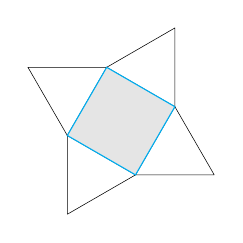
\begin{tikzpicture}[scale=.5]
		\tkzDefPoints{-1/0/A,1/0/A1,0/0/O}
	%	\tkzDrawPoints[color=black,size=2pt](A,A1,O)
		\tkzDefPointBy[rotation=center A angle 60](A1)
		\tkzGetPoint{B}
%		\tkzDrawPoints[color=black,size=2pt](B)
		\tkzDrawPolygon(A,A1,B)
		\tkzDefPointBy[rotation=center B angle -90](A)
		\tkzGetPoint{C}
	%	\tkzDrawPoints[color=black,size=2pt](C)
		\tkzDefPointBy[rotation=center A angle 90](B)
		\tkzGetPoint{D}
	%	\tkzDrawPoints[color=black,size=2pt](D)
	
		\tkzDefPointBy[rotation=center B angle -60](C)
		\tkzGetPoint{B1}
	%	\tkzDrawPoints[color=black,size=2pt](B1)
		\tkzDrawPolygon(B,B1,C)
		\tkzDefPointBy[rotation=center C angle -60](D)
		\tkzGetPoint{C1}
	%	\tkzDrawPoints[color=black,size=2pt](C1)
		\tkzDrawPolygon(C,C1,D)
		\tkzDefPointBy[rotation=center D angle -60](A)
		\tkzGetPoint{D1}
	%	\tkzDrawPoints[color=black,size=2pt](D1)
		\tkzDrawPolygon(D,D1,A)
	\tkzFillPolygon[draw=cyan,fill=gray!20](A,B,C,D)
	\end{tikzpicture}
	
\end{document}